\documentclass[article,shortnames]{jss}
\usepackage{float}
\usepackage[]{media9}

\usepackage{tcolorbox}% http://ctan.org/pkg/tcolorbox
\definecolor{frameCol}{rgb}{0.122, 0.435, 0.698}% Rule colour
\definecolor{bgndCol}{rgb}{.66,.66,.66}% Rule colour
\makeatletter
\newcommand{\mybox}[1]{%
  \setbox0=\hbox{#1}%
  \setlength{\@tempdima}{\dimexpr\wd0+13pt}%
  \begin{tcolorbox}[colframe=frameCol,colback=bgndCol,boxrule=0.5pt,arc=4pt,
      left=6pt,right=6pt,top=6pt,bottom=6pt,boxsep=0pt,width=\@tempdima]
    #1
  \end{tcolorbox}
}
\makeatother

%%%%%%%%%%%%%%%%%%%%%%%%%%%%%%
%% declarations for jss.cls %%%%%%%%%%%%%%%%%%%%%%%%%%%%%%%%%%%%%%%%%%
%%%%%%%%%%%%%%%%%%%%%%%%%%%%%%

%% almost as usual
\author{Lindsay Rutter\\Iowa State University \And 
        Susan VanderPlas\\Iowa State University \And
        Dianne Cook\\Monash University\And
        Michelle A. Graham\\Iowa State University}
\title{\pkg{ggenealogy}: An \proglang{R} Package for Visualizing Genealogical Data}

%% for pretty printing and a nice hypersummary also set:
\Plainauthor{Lindsay Rutter, Susan VanderPlas, Di Cook} %% comma-separated
\Plaintitle{ggenealogy: An R Package for Visualizing Genealogical Data} %% without formatting
\Shorttitle{\pkg{ggenealogy}: An \proglang{R} Package for Visualizing Genealogical Data} %% a short title (if necessary)

%% an abstract and keywords
\Abstract{
  This paper introduces \pkg{ggenealogy} (\citealt{ggen}), a developing \proglang{R} software package that provides tools for searching through genealogical data, generating basic statistics on their graphical structures using parent and child connections, and displaying the results. It is possible to draw the genealogy in relation to variables related to the nodes, and to determine and display the shortest path distances between the nodes. Production of pairwise distance matrices and genealogical diagrams constrained on generation are also available in the visualization toolkit. The tools are being tested on a dataset with milestone cultivars of soybean varieties (\citealt{soybean}) as well as on a web-based database of the academic genealogy of mathematicians (\citealt{mgp}). The software package is currently available on the Comprehensive \proglang{R} Archive Network.}

\Keywords{genealogy, data visualization, statistical graphics, exploratory data analysis, interactive, \proglang{R}}
\Plainkeywords{genealogy, data visualization, statistical graphics, exploratory data analysis, interactive, R} %% without formatting
%% at least one keyword must be supplied

%% publication information
%% NOTE: Typically, this can be left commented and will be filled out by the technical editor
%% \Volume{50}
%% \Issue{9}
%% \Month{June}
%% \Year{2012}
%% \Submitdate{2012-06-04}
%% \Acceptdate{2012-06-04}

%% The address of (at least) one author should be given
%% in the following format:
\Address{
  Lindsay Rutter\\
  Bioinformatics and Computational Biology Program\\
  Iowa State University\\
  2014 Molecular Biology Building\\
  Ames, IA, 50011, United States of America\\
  E-mail: \email{lrutter@iastate.edu}\\
  URL: \url{https://github.com/lrutter/}\\

  Susan VanderPlas\\
  Department of Statistics\\
  Iowa State University\\
  2413 Snedecor Hall\\
  Ames, IA, 50011, United States of America\\
  E-mail: \email{srvanderplas@gmail.com}\\
  URL: \url{https://github.com/srvanderplas/}\\
  
  Dianne Cook\\
  Department of Econometrics and Business Statistics\\
  Monash University\\
  E869 Menzies Building\\
  20 Chancellors Walk\\
  Clayton, VIC 3800, Australia\\
  E-mail: \email{dicook@monash.edu}\\
  URL: \url{https://github.com/dicook/}\\

  Michelle Graham\\
  USDA-Agriculture Research Service, Corn Insects and Crop Genetics Research Unit\\
  Department of Agronomy, Iowa State University\\
  1565 Agronomy Building\\
  Ames, IA, 50011, United States of America\\
  E-mail: \email{michelle.graham@ars.usda.gov}
}

%% It is also possible to add a telephone and fax number
%% before the e-mail in the following format:
%% Telephone: +43/512/507-7103
%% Fax: +43/512/507-2851

%% for those who use Sweave please include the following line (with % symbols):
%% need no \usepackage{Sweave.sty}

%% end of declarations %%%%%%%%%%%%%%%%%%%%%%%%%%%%%%%%%%%%%%%%%%%%%%%

\begin{document}

%% include your article here, just as usual
%% Note that you should use the \pkg{}, \proglang{} and \code{} commands.

%% \section[About Java]{About \proglang{Java}}
%% Note: If there is markup in \(sub)section, then it has to be escape as above.

\section{Introduction}

Genealogy is the study of parent-child relationships. By tracing through parent-child lineages, genealogists can study the histories of features that have been modified over time. Comparative geneticists, computational biologists, and bioinformaticians commonly use genealogical tools to better understand the histories of novel traits arising across biological lineages. For example, desirable modifications in crops could include an increase in protein yield or an increase in disease resistance, and genealogical structures could be used to assess how these desirable traits developed. At the same time, genealogical lineages can also be used to assess detrimental features, such as to determine the origin of hazardous traits in rapidly-evolving viruses.

Genealogical structures can also serve as informative tools outside of a strict biological sense. For instance, we can trace mentoring relationships between students and dissertation supervisors with the use of academic genealogies. This can allow us to understand the position of one member in the larger historical picture of academia, and to accurately preserve past relationships for the knowledge of future generations. Similarly, linguistic genealogies can be used to decipher the historical changes of vocabulary and grammatical features across related languages. In short, there is a diverse array of disciplines that can elicit useful information about features of interest by using genealogical data.

In all these examples, the genealogical relationships can be represented visually. Access to various types of plotting tools can allow scientists and others to more efficiently and accurately explore features of interest across the genealogy. We introduce here a developing visualization toolkit that is intended to assist users in their exploration and analysis of genealogical structures. In this paper, we demonstrate the main tools of the software package \pkg{ggenealogy} using two example genealogical datasets, one of soybean cultivars (\citealt{soybean}) and the other of academic mathematicians (\citealt{mgp}).

\section{Available Software}

Publishing in the open source \proglang{R} statistical programming language allows for tools to be distributed and modified at ease, encourages cross-platform collaboration, and provides a foundation for effective and aesthetic data visualization from the grammar of graphics. There are several useful \proglang{R} packages that offer tools for analyzing and visualizing genealogical datasets. Here, we introduce these packages, and emphasize the new features that \pkg{ggenealogy} brings to this collection of work.

The \proglang{R} package \proglang{pedigree} is named after the standardized chart used to study human family lines, and sometimes used to select breeding of animals, such as show dogs (\citealt{ped}). This package does provide tools that perform methods on parent-child datasets, such as rapidly determining the generation count for each member in the pedigree. However, it does not provide any visualization tools.

Another \proglang{R} package called \proglang{kinship2} does produce basic pedigree charts (\citealt{kin}). In Figure \ref{fig:kinshipFig}, we provide an example pedigree chart from the \proglang{kinship2} package vignette. This pedigree chart adheres to the standard set of symbols used for visualizing genealogical structures: Males are represented with squares and females with circles. Parents are connected to each other by horizontal lines, and to their children by vertical lines. Siblings are connected by horizontal sibship lines. Even though this standard pedigree chart creates powerful charts that can be applied across many applications, it cannot provide unequivocal information in situations where inter-generational breeding occurs, as is often the case in agronomic genealogical lineages.

We demonstrate how the standardized pedigree charts in the \proglang{kinship2} package generate ambiguous results in such scenarios by superimposing a hypothetical inter-generational breeding case in Figure \ref{fig:kinshipFig}. In that figure, each generation is defined by its position on the vertical axis, with the first generation containing individuals 201 and 202. We superimposed green-highlighted individual 215 onto the pedigree chart for explanatory purposes. Its parents are individuals 201 and 206, which are from generations one and two, respectively, and have a parent-child relationship between themselves. As an offspring of a parent-child relationship, individual 215 is both a second and third generation individual. Hence, individual 215 should be displayed in both second and third generational positions on the vertical axis. However, standard pedigree tools only allow for an individual to be displayed once. As a result, in special cases where inter-generational breading occurs, such as in agronomic applications, standardized tools for visualizing genealogical information ambiguously portray the genealogical dataset.

\begin{figure}[H]
    \centering
    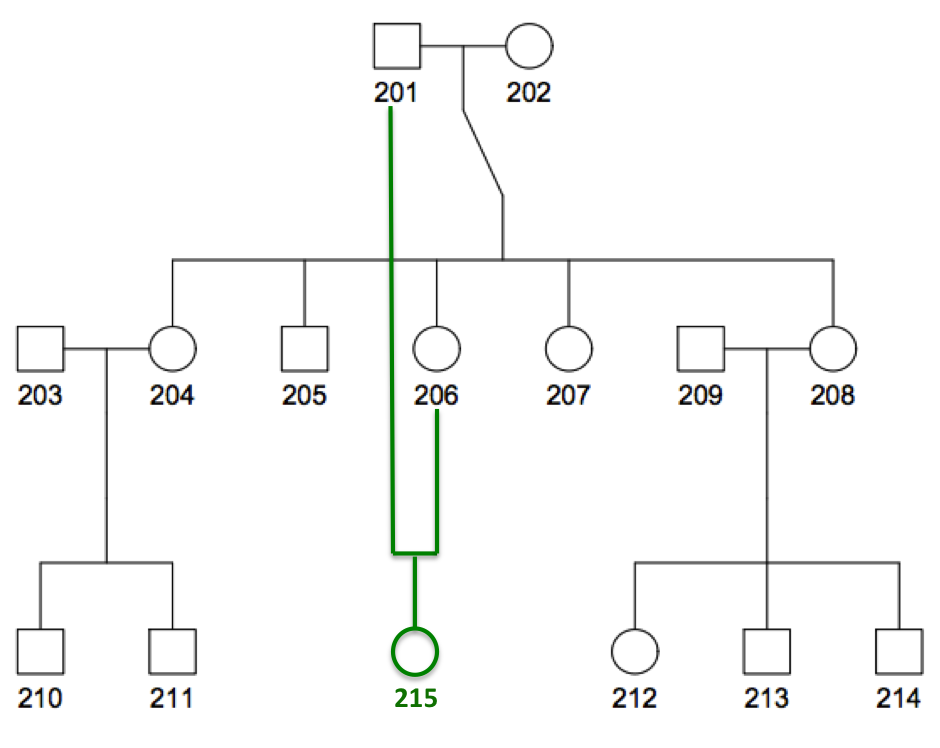
\includegraphics[width=0.65\textwidth]{kinshipFig}
    \caption{Example pedigree chart from the \proglang{kinship2} package, where the vertical axis denotes generation count. We superimposed green-highlighted individual 215 for explanatory purposes. As an offspring of a parent-child relationship, individual 215 is both a second and third generation individual. Hence, it should be displayed twice on the vertical axis, once for each of its generation counts. However, standard pedigree tools only allow for an individual to be displayed once, leading to ambiguous portrayal of the genealogical dataset.}
    \label{fig:kinshipFig}
\end{figure}

In addition, popular graph drawing software such as \proglang{GraphViz} and \proglang{Cytoscape} can be used to visualize genealogical structures (\citealt{graphvizCit}, \citealt{cytoscapeCit}). Graphs are defined as objects with sets of nodes and edges, where sets indicate that their comprised elements cannot be repeated. In other words, graphical structures do not allow for repeated nodes, and hence, as is the case with the aforementioned \proglang{R} packages, these popular graph plotting software cannot precisely portray the genealogical dataset in cases of inter-generational breeding.

We again illustrate this problem in Figure \ref{fig:Graph} with an example genealogy using popular graph drawing software like \proglang{GraphViz} and \proglang{Cytoscape}. Here, generation count is denoted by the vertical axis. As was shown in Figure \ref{fig:kinshipFig}, here too we superimpose a green node that has parents from two different generations. This green node is both a second and third generation individual, and should be displayed in both corresponding generation positions on the vertical axis. However, standard graph visualization tools only allow for a given node to be displayed once. As a result, this green node must be ambiguously positioned in either the second or third generation position; in the figure, it is denoted as a third generation individual. In Section \ref{remedy}, we will demonstrate \pkg{ggenealogy} plots that can remedy these problems.

\begin{figure}[H]
    \centering
    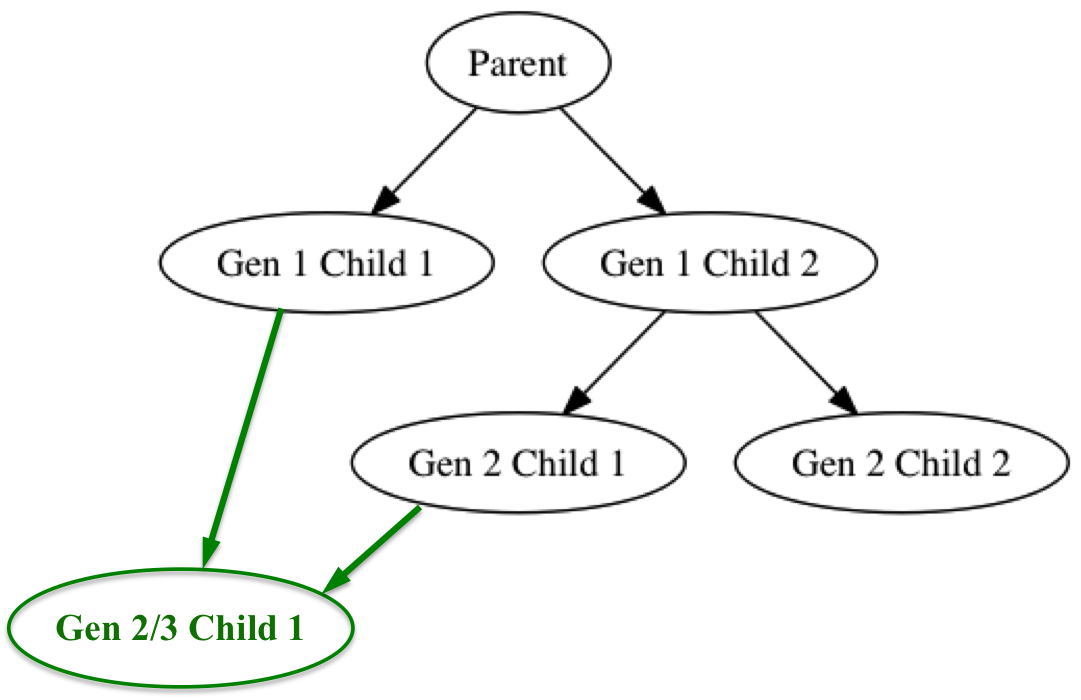
\includegraphics[width=0.6\textwidth]{Graph}
    \caption{Example genealogical display using popular graph software like \proglang{GraphViz} and \proglang{Cytoscape}, with generation count denoted by the vertical axis. As was shown in Figure \ref{fig:kinshipFig}, the green node has parents from two different generations, and hence must be ambiguously positioned as one of two generation counts.}
    \label{fig:Graph}
\end{figure}

\section{Example Datasets}
\label{exData}

The \pkg{ggenealogy} package comes with two example datasets, one comprises a soybean genealogy and the other comprises an academic statistician genealogy. We will introduce both example datasets in this paper to demonstrate some of the tools available in the software.

\subsection{Soybean Genealogy}

We start with the soybean genealogy, which is available as a data frame structure with 390 rows and five columns. These data were collected from field trials, genetic studies, and United States Department of Agriculture (USDA) bulletins, and date as early as the first decade of the 1900s. They contain information on the copy number variants, single nucleotide polymorphisms, and protein content for each of the varieties, although we removed that information for a succinct example dataset. In this context, the software could ideally be used by agronomists who wish to study how soybean varieties are related. By referencing the visualization of the genealogical structure, these scientists may better understand genetic testing results - in this particular dataset, in terms of copy number variants, single nucleotide polymorphisms, protein content, and yield - and use that knowledge in future breeding decisions.

Each row contains information about a particular child soybean variety, including the name of the child, its yield, the year it was released, whether or not its release year was imputed, and the name of its parent. It should be noted that it typically requires many crosses over the span of one to two decades to develop a new variety that has introduced a desired trait and/or removed an undesired trait. Hence, the release year variable in this dataset represents the year in which the variety was released to the public after its development period. While the name of the child is required, the other four columns can have missing values (which are represented in \proglang{R} with the symbol NA for ``not available"). As a result, while each row does contain information about a particular child soybean variety, whether or not a given row also contains information about a parent-child relationship between a pair of soybeans depends on whether or not the parent column has a missing value.

In total, there are 230 soybean varieties in the dataset, 206 of which are children and 165 of which are parents. There are soybeans that are both children and parents. Of the children, 156 have two parents, 28 have one parent, and 22 have zero parents. There are 340 parent-child relationships in the dataset.

We can load the example dataset of soybean genealogy (\code{sbGeneal}) and examine its structure. 

\begin{CodeChunk}
\begin{CodeInput}
R> install.packages("ggenealogy")
R> library("ggenealogy")
R> data(sbGeneal)
R> str(sbGeneal)
\end{CodeInput}
\begin{CodeOutput}
'data.frame':	390 obs. of  5 variables:
 $ child       : chr  "5601T" "Adams" "A.K." "A.K. (Harrow)" ...
 $ year        : num  1981 1948 1910 1912 1968 ...
 $ yield       : int  NA 2734 NA 2665 NA 2981 2887 2817 NA NA ...
 $ year.imputed: logi  TRUE FALSE TRUE FALSE FALSE FALSE ...
 $ parent      : chr  "Hutcheson" "Dunfield" NA "A.K." ...
\end{CodeOutput}
\end{CodeChunk}

\subsection{Academic Genealogy of Statisticians}

The \pkg{ggenealogy} package also comes with an academic genealogy of statisticians; this dataset is in the form of a data frame with 8165 rows and six columns. To develop this later dataset, we contacted the \citealt{mgp}, a web-based database for the genealogy of academic mathematicians. This database, which currently contains almost 200,000 entries, is a service of the North Dakota State University Department of Mathematics and the American Mathematical Society. The Mathematics Genealogy Project contact provided us a Structured Query Language (SQL) export, and we used PostgreSQL to query the database (\citealt{psql}).

Each entry in the database contained 26 variables pertaining to an individual who received a graduate-level academic degree in mathematics. One of these variables was called ``msc" (Mathematics Subject Classification), and we selected only those entries that contained a value of 62 for this variable (coded as ``Statistics"). Furthermore, we only retained entries that had a parent if that parent was also in the field of ``Statistics". Hence, in our parent-child relationships, both the child and the parent received postbaccalaureate degrees in statistics, and the parent was the academic advisor to the child. This process resulted in 8995 entries, which we reduced to 8165 entries by removing duplicate entries. With the final data frame of 8165 entries, we only maintained six of the original 26 variables. 

Each row of the final data frame contains information about a particular child who received a graduate-level academic degree in statistics, including the name of the child, the year the child obtained the degree, the country and school from which the child obtained the degree, the thesis title of the degree awarded to the child, and the name of its parent. There are no missing values for the country and school from which the child received its degree or the name of the child; however, some of the years contain missing values (NA), and some of the parent and thesis names contain empty strings (``"). As a result, while each row does contain information about a particular child, whether or not a row also contains information about a parent-child relationship between a pair of academic statisticians depends on whether or not the parent column has an empty string.
 
In total, there are 7122 individuals in the dataset, 7122 of which are children and 872 of which are parents. Every parent is also a child, but not every child is also a parent. Of the children, two have four parents, ten have three parents, 226 have two parents, 2801 have one parent, and 4083 have no parents. There are 3291 parent-child relationships in the dataset.

We can load the example dataset of academic genealogy of statisticians (\code{statGeneal}) and examine its structure. 

\begin{CodeChunk}
\begin{CodeInput}
R> data(statGeneal)
R> dim(statGeneal)
\end{CodeInput}
\begin{CodeOutput}
[1] 8165    6
\end{CodeOutput}
\begin{CodeInput}
R> colnames(statGeneal)
\end{CodeInput}
\begin{CodeOutput}
[1] "child"   "parent"  "year"    "country" "school"  "thesis"
\end{CodeOutput}
\end{CodeChunk}

\section{Genealogical Input Format}

As is the case with both example data files introduced above, \pkg{ggenealogy} requires that the genealogy input file is a data frame structure with at least two columns. One column must be labeled ``child", and each case in that column must be of type character. The other column must be labeled ``parent," and each case in that column must either be of type character, type NA, or type ``". At this point, any \pkg{ggenealogy} plot that only requires information about parent-child relationships can be used.

However, some \pkg{ggenealogy} plots also make use of quantitative variable values associated with individuals in the genealogy. For these plots, the input data frame should also contain a third column. In both example data files, this column is labeled ``year," and each case in that column can either be of type numeric, type NA, or type ``". At this point, any \pkg{ggenealogy} plot can be used.

\section{Generating a Graphical Object}

Most functions in the \pkg{ggenealogy} software package require an input parameter of a graph structure. Therefore, as a preprocessing step, we must first convert our original data frame structure into a graph structure. Below, we read in the \proglang{R} data file \code{sbGeneal} that is included in the package as a sample data set of soybean genealogy.

We now convert it into an \pkg{igraph} object (\citealt{igraph}) \code{sbIG} using the function \code{dfToIG()}.

\begin{CodeChunk}
\begin{CodeInput}
R> sbIG <- dfToIG(sbGeneal)
R> sbIG
\end{CodeInput}
\begin{CodeOutput}
IGRAPH UNW- 230 340 -- 
+ attr: name (v/c), weight (e/n)
+ edges (vertex names):
 [1] 5601T    --Hutcheson        Adams    --Dunfield        
 [3] A.K.     --A.K. (Harrow)    Altona   --Flambeau        
 [5] Amcor    --Amsoy 71         Adams    --Amsoy           
 [7] Amsoy 71 --C1253            Anderson --Lincoln         
 [9] Bay      --York             Bedford  --Forrest         
[11] Beeson   --Kent             Blackhawk--Richland        
[13] Bonus    --C1266R           Bradley  --J74-39          
[15] Bragg    --Jackson          Bragg    --Bragg x D60-7965
+ ... omitted several edges
\end{CodeOutput}
\end{CodeChunk}

There are many statistics about the \code{sbGeneal} dataset that we may wish to know that cannot easily be obtained through images and tables. The package function \code{getBasicStatistics()} can be called, using the \code{sbIG} object as input. This will return a list of common graph theoretical measurements regarding the genealogical structure. For instance, is the whole structure connected? If not, how many separated components does it contain? In addition to these statistics, the \code{getBasicStatistics()} function will also return the number of nodes, the number of edges, the average path length, the graph diameter, and other graph theoretical information.

\begin{CodeChunk}
\begin{CodeInput}
R> getBasicStatistics(sbIG)
\end{CodeInput}
\begin{CodeOutput}
$isConnected
[1] FALSE

$numComponents
[1] 11

$avePathLength
[1] 5.333746

$graphDiameter
[1] 13

$numNodes
[1] 230

$numEdges
[1] 340

$logN
[1] 5.438079
\end{CodeOutput}
\end{CodeChunk}

\section{Plotting a Shortest Path}

With soybean lineages, it may be useful for soybean breeders to track how two varieties are related to each other via parent-child relationships. Then, any dramatic changes in yield and other measures of interest between the two varieties can be traced across their genetic timeline. The \pkg{ggenealogy} package allows users to select two varieties of interest, and determine the shortest pathway of parent-child relationships between them, using the \code{getPath()} function. This will return a list that contains the variety names and their years in the path.

\begin{CodeChunk}
\begin{CodeInput}
R> pathTN <- getPath("Tokyo", "Narow", sbIG, sbGeneal)
R> pathTN
\end{CodeInput}
\begin{CodeOutput}
$pathVertices
[1] "Tokyo"    "Volstate" "Jackson"  "R66-873"  "Narow"   

$yearVertices
[1] "1907"   "1942"   "1954.5" "1971.5" "1985" 
\end{CodeOutput}
\end{CodeChunk}

The returned path object can then be plotted using the \code{plotPath()} function.

\begin{Code}
R> plotPath(pathTN)
\end{Code}

\begin{figure}[h]
    \centering
    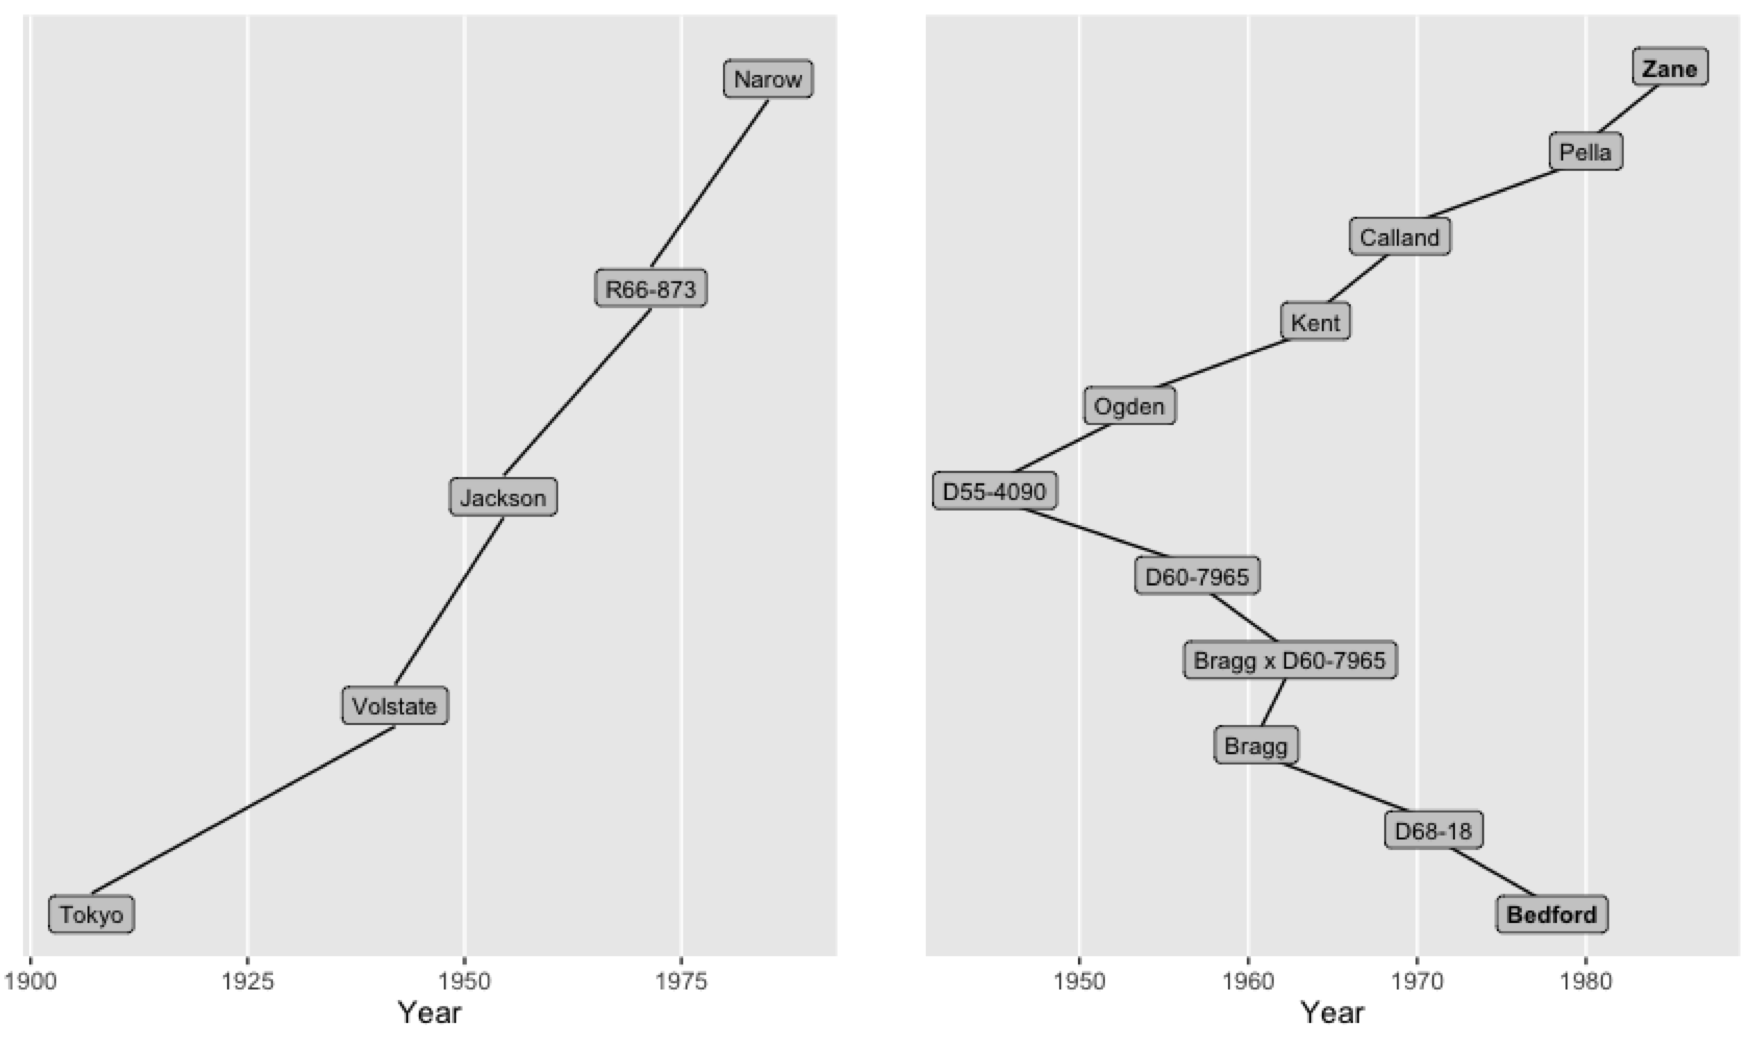
\includegraphics[width=\textwidth]{pathTNZB}
    \caption{Left: The shortest path between varieties Tokyo and Narow is strictly composed of a unidirectional sequence of parent-child relationships. Right: The shortest path between varieties Zane and Bedford is not strictly composed of unidirectional parent-child relationships; they instead have a cousin-like relationship.}
    \label{fig:pathTNZB}
\end{figure}

This produces a visual that informs users of all the varieties involved in the shortest path between the two varieties of interest (see left half of Figure \ref{fig:pathTNZB}). In this plot, the release year of all varieties involved in the path are indicated on the horizontal axis, while the vertical axis has no meaning other than to simply to display the labels evenly spaced vertically. The shortest path between varieties \code{Tokyo} and \code{Narow} is composed of a unidirectional series of parent-child relationships, with \code{Tokyo} as the starting ancestor in the early 1900s, \code{Narow} as the most recent descendent in the mid 1980s, and three varieties in between.

Next, we can run the same set of functions on a different pair of varieties. First, a call to the \pkg{ggenealogy} function \code{getYear()} indicates that variety \code{Bedford} was released in 1978 and variety \code{Zane} in 1985.

\begin{CodeChunk}
\begin{CodeInput}
R> getYear("Bedford", sbGeneal)
\end{CodeInput}
\begin{CodeOutput}
[1] 1978
\end{CodeOutput}
\begin{CodeInput}
R> getYear("Zane", sbGeneal)
\end{CodeInput}
\begin{CodeOutput}
[1] 1985
\end{CodeOutput}
\end{CodeChunk}

We can then create a plot showing the shortest path between these two varieties of interest. As this is a longer path, we may also consider setting the \code{fontFace} variable of the \code{plotPath()} to a value of 2, indicating we wish to boldface the two varieties of interest.

\begin{Code}
R> pathBZ <- getPath("Bedford", "Zane", sbIG, sbGeneal)
R> plotPath(pathBZ, fontFace = 2)
\end{Code}

The resulting plot (right half of Figure \ref{fig:pathTNZB}) allows us to quickly determine that \code{Bedford} is not a parent, grandparent, or any great grandparent of \code{Zane}. Instead, we see that these two varieties are not related through a unidirectional parent-child lineage, but instead have a cousin-like relationship. The oldest common ancestor between \code{Zane} and \code{Bedford} is the variety \code{D55-4090}, which was released in the mid 1940s.

Furthermore, as determined by the figure, for both \code{Zane} and \code{Bedford}, there are four varieties of unidirectional parent-child relationships between each of them and their common ancestor \code{D55-4090}. Hence, any feature of interest that differentiates \code{Zane} and \code{Bedford} (protein content, yield, disease resistance, etc.) can also be examined across these two separate lineage histories.

\section{Superimposing Shortest Path on Tree}

Now that we can create path objects, we may wish to know how those paths are positioned compared to the entire genealogical lineage. For instance, of the documented soybean cultivar lineage varieties, where does the shortest path between two varieties of interest exist? Are these two varieties older compared to the overall data structure? Are they newer? Or, do they span the entire structure, and represent two extreme ends of documented time points?

There is a function available in the \pkg{ggenealogy} package \code{plotPathOnAll()} that can allow users to quickly visualize their path of interest superimposed over all varieties and edges present in the whole data structure. Here we will produce a plot of the shortest path between varieties \code{Tokyo} and \code{Narow} across the entire dataset, as is displayed in Figure \ref{fig:plotTNBin3}.

\begin{Code}
R> plotPathOnAll(pathTN, sbGeneal, sbIG, binVector = 1:3, pathEdgeCol = "red",
  nodeSize = 2.5, pathNodeSize = 4) + ggplot2::theme(axis.text = ggplot2::
  element_text(size = 12), axis.title = ggplot2::element_text(size = 12))
\end{Code}

\begin{figure}%[h]
    \centering
    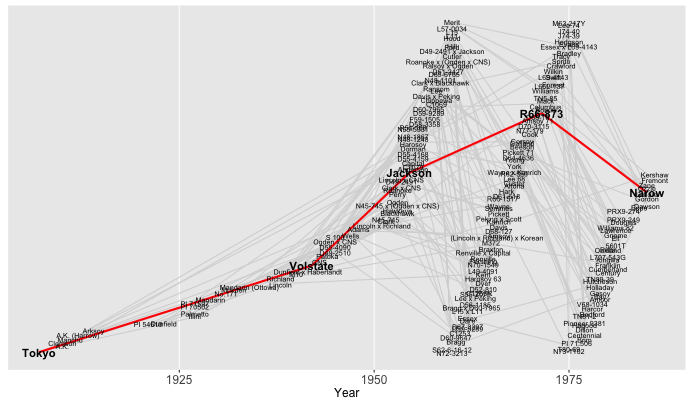
\includegraphics[width=\textwidth]{plotTNBin3}
    \caption{The shortest path between Tokyo and Narow, superimposed over the data structure, using a bin size of 3.}
    \label{fig:plotTNBin3}
\end{figure}

In the code above, syntax from the \pkg{ggplot2} package was appended to the \code{plotPathOnAll()} function; this can be done for most \pkg{ggenealogy} functions (\citealt{ggplot2}). While the first three explicit parameters have been introduced earlier in this paper, the fourth parameter (\code{binVector}) requires some explanation. The motivation of the \code{plotPathOnAll()} function is to write node labels on a plot, with the center of each node label constricted on the horizontal axis to its quantitative variable of interest (in this case, year of release). As is the case for the plots before, the vertical axis has no meaning other than providing a plotting area in which to draw the node labels. Unfortunately, for large datasets, this motivation can be a difficult task because the text labels of the varieties can overlap if they are assigned a similar y coordinate, have a similar year (x coordinate), and have long text labels (width of x coordinate).

For each variety, the x coordinate (year) and width of the x coordinate (text label width) cannot be altered, as they provide useful information. However, for each variety, the y coordinate is arbitrary. Hence, in an attempt to mitigate text overlapping, the \code{plotPathOnAll()} function does not randomly assign the y coordinate. Instead, it allows users to partially control the y coordinates with a user-determined number of bins (\code{binVector}).

If the user decides to produce a plot using three bins, as in the example code above, then the varieties are all grouped into three bins based on their year values. In other words, there will be bin 1 (the ``oldest bin") which includes the one-third of varieties with the oldest years of release, bin 2 (the ``middle bin"), and bin 3 (the ``youngest bin"). Then, in order to decrease text overlap, the consecutively increasing y-axis coordinates are alternatively assigned to the three bins (For example: bin 1, bin 2, bin 3, bin 1, bin 2, bin 3, ...) repeatedly until all varieties are addressed. This algorithm means that for any pair of varieties within a given bin, there are exactly two other varieties vertically separating them.

In the code above, \code{binVector} was assigned a value of 3, and \code{pathEdgeCol} was assigned a value of ``red". Additionally, we specified a size of 2.5 for the non-path node test using the \code{nodeSize} parameter, and a size of 4 for the path node text using the \code{pathNodeSize} parameter. There are several other parameters in the \code{plotPathOnAll()} function, which can be read in more detail using the help command.

This code resulted in Figure \ref{fig:plotTNBin3}, where we see that edges not on the path of interest are thin and gray by default, whereas edges on the path of interest are bolded by default. We also see that variety labels in the path of interest are boldfaced by default. Figure \ref{fig:plotTNBin3} presents useful information: We immediately gather that the path of interest does span most of the years of the data structure. In fact, \code{Tokyo} appears to be the oldest variety in the dataset, and \code{Narow} appears to be one of the youngest varieties. We can also determine that the majority of varieties were released between 1950 and 1970.

However, Figure \ref{fig:plotTNBin3} has significant empty spaces between the noticeably distinct bins, whereas almost all text labels are overlapping, thereby decreasing their readability. To force text labels into these spaces, the user may consider using a larger number of bins. Hence, we next examine a bin size of 6 to create Figure \ref{fig:plotTNBin6}.

\begin{Code}
R> plotPathOnAll(pathTN, sbGeneal, sbIG, binVector = 1:6, pathEdgeCol =
  "seagreen2", nodeSize = 1, pathNodeSize = 3)
\end{Code}

\begin{figure}[H]
    \centering
    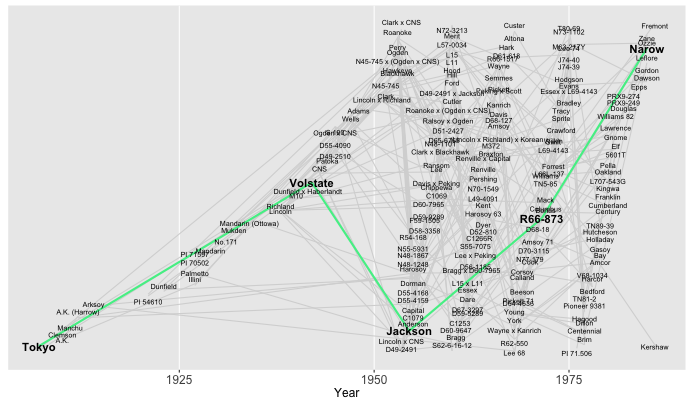
\includegraphics[width=\textwidth]{plotTNBin6}
    \caption{The shortest path between Tokyo and Narow, superimposed over the data structure, using a bin size of 6.}
    \label{fig:plotTNBin6}
\end{figure}

We can immediately see that Figure \ref{fig:plotTNBin6} more successfully mitigates text overlap compared to Figure \ref{fig:plotTNBin3}. We can also confirm what we saw in the previous plot that indeed most varieties were released between 1950 and 1970, and any textual overlap is confined to this range of years.

\section{Plotting Ancestors and Descendants by Generation}
\label{remedy}

The most novel visual function in \pkg{ggenealogy}, \code{plotAncDes()} allows users to view the ancestors and descendants of a given variety. The inputted variety is highlighted in the center of the plot, ancestors are displayed to the left of the center, and descendants are displayed to the right of the center. The further from the center that a variety is located, the more generations that variety is distanced from the centered variety of interest.

This particular \pkg{ggenealogy} tool is unique because most available genealogy and graph visualization software do not allow for repeated labels. It is a useful tool because, as was demonstrated in Figures \ref{fig:kinshipFig} and \ref{fig:Graph}, some genealogical datasets require repeated node labels if they are to be visualized by generation counts. Indeed, our example soybean genealogy is one such dataset.

To demonstrate this tool, we will create a plot of the ancestors and descendants of the variety \code{Lee}. We specify that the maximum number of ancestor and descendant generations are both 6, and that the text of the variety of interest is highlighted in blue:

\begin{Code}
R> plotAncDes("Lee", sbGeneal, mAnc = 6, mDes = 6, vCol = "blue")
\end{Code}

This generates the top plot of Figure \ref{fig:Lee}. We notice that \code{Lee} has 3 generations of ancestors and 5 generations of descendants. We also notice that some varieties are repeated in the plot, which is a unique feature provided by \pkg{ggenealogy}. For example, the variety \code{5601T} is represented four times - once as a third generation descendant of \code{Lee}, once as a fourth generation descendant of \code{Lee}, and twice as a fifth generation descendant of \code{Lee}. The variety \code{5601T} was repeated multiple times because there are multiple paths between \code{Lee} and \code{5601T}. For explanation purposes, all paths between \code{Lee} and \code{5601T} were manually highlighted in blue.

\begin{figure}[H]
    \centering
    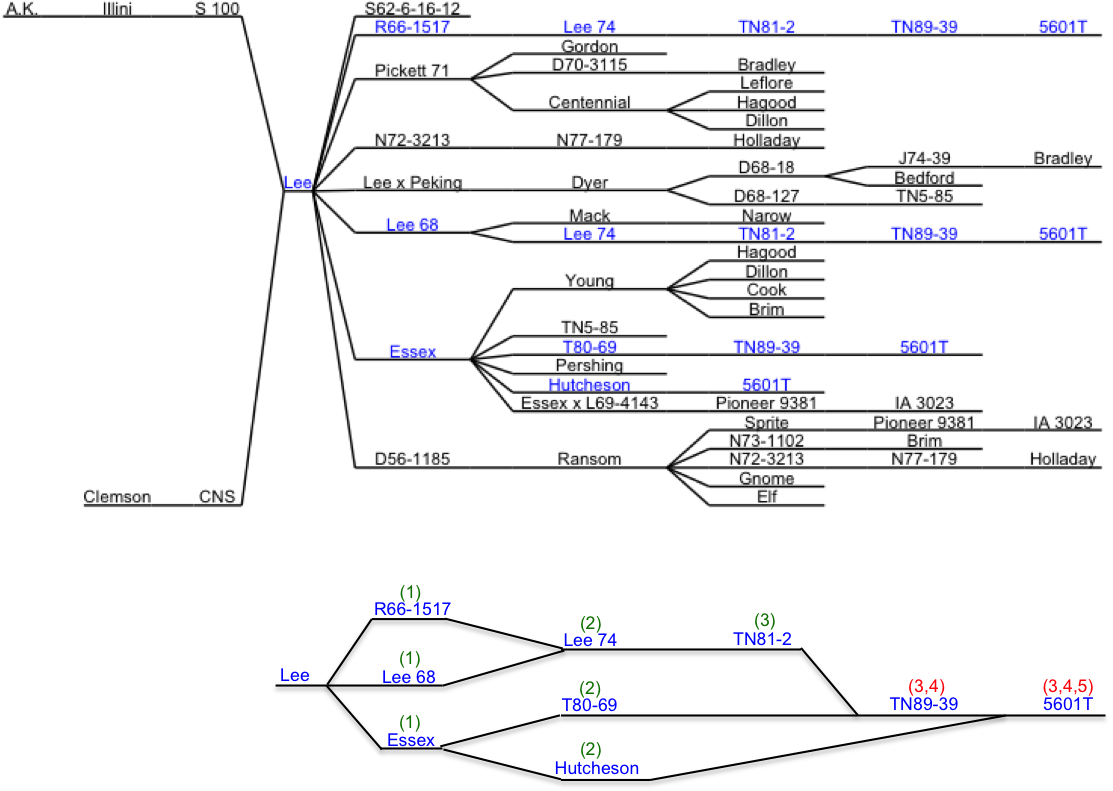
\includegraphics[width=\textwidth]{LeeAD3}
    \caption{Top: All ancestors and descendants of the variety Lee are shown in this ggenealogy plot. Bottom: We now attempt to mimic the blue paths in the ggenealogy plot on the top, only now nodes cannot be repeated. The parenthetical numbers above each node represents the set of generation counts that node is away from the center node Lee. The presence of red parentheses indicate that the plot on the bottom ambiguously display the example soybean genealogy in the way that the ggenealogy plot on the top can accomplish.}
    \label{fig:Lee}
\end{figure}

The bottom plot of Figure \ref{fig:Lee} is not an output plot of \pkg{ggenealogy}. Instead, it was simply created for didactic purposes. Here, the paths that were manually highlighted in blue in the top plot produced by \pkg{ggenealogy} are shown again, only now nodes cannot be repeated. The parenthetical number above each node represents the set of generation counts distancing that node from the center node \code{Lee}; green parentheses indicate that the node could be successfully placed in one horizontal position, but red parentheses indicate that the node could not be successfully placed in one horizontal position. We see that node \code{TN89-39} cannot simultaneously be represented as both a third and fourth descendent of node \code{Lee}, and node \code{5601T} cannot simultaneously be represented as a third, fourth, and fifth descendent of node \code{Lee}. Hence, without allowing nodes to repeat, this dataset cannot be presented in the graph on the bottom as it can be in the \pkg{ggenealogy} graph on the top. This is a current limitation in other genealogy and graphical software that \pkg{ggenealogy} can now provide.

\section{Plotting Distance Matrix}

It may also be of interest to generate matrices where the colors indicates a variable between all pairwise combinations of inputted varieties. The package \pkg{ggenealogy} also provides a function \code{plotDegMatrix()} for that purpose. We can demonstrate this function with the variable being the shortest path degree between a given pair of varieties. The shortest path degree is calculated as the smallest number of parent-child edges needed to traverse between two varieties of interest. For instance, in Figure \ref{fig:pathTNZB}, the shortest path degree between \code{Tokyo} and \code{Narow} is four and the shortest path degree between \code{Bedford} and \code{Zane} is ten.

Here we generate a distance matrix for a set of 10 varieties, setting the x-label and y-label as ``Variety" and the legend label as ``Degree". In this example, we add \pkg{ggplot2} functionality to specify that pairs with small degrees are white, while those with large degrees are dark green, as well as to specify the text size of the legend title and label.

\begin{Code}
>R varieties <- c("Brim", "Bedford", "Calland", "Dillon", "Hood", "Narow",
  "Pella", "Tokyo", "Young", "Zane")
>R plotDegMatrix(varieties, sbIG, sbGeneal, "Variety", "Variety", "Degree") +
  ggplot2::scale_fill_continuous(low = "white", high = "darkgreen") +
  ggplot2::theme(legend.title = ggplot2::element_text(size = 15), legend.text
  = ggplot2::element_text(size = 15))
\end{Code}

This creates the plot in Figure \ref{fig:degMatrix}. We see that the degree of the shortest path between varieties \code{Bedford} and \code{Zane} is 10, which is consistent with what we saw earlier in Figure \ref{fig:pathTNZB}. However, we now also see that a shortest path degree of 10 may be considered relative to the rest of this dataset.

\begin{figure}[h]
    \centering
    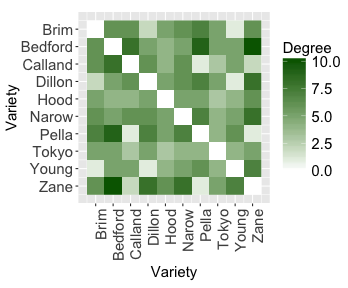
\includegraphics[width=0.5\textwidth]{degMatrix}
    \caption{The shortest path degree matrix between ten varieties of interest.}
    \label{fig:degMatrix}
\end{figure}

\section{Academic Genealogy of Statisticians}

The \pkg{ggenealogy} package comes with two example datasets, and while we have introduced the plant breeding genealogy, we have yet to introduce the academic genealogy. As was demonstrated in Section \ref{exData}, every parent in the academic genealogy is also a child, and some children in the academic genealogy have more than two parents. Neither of these features was the case in the plant breeding genealogy. Additionally, the academic genealogy is much larger than the plant breeding genealogy. Some of these differences may affect how one would approach \pkg{ggenealogy} plotting tools. For this reason, we will now demonstrate some of the \pkg{ggenealogy} plotting tools we already introduced, only now applied to the academic genealogy. 

The ability to plot ancestors and descendants by generation was demonstrated using the plant breeding genealogy in Figure \ref{fig:Lee}. As we believe this is the most novel plotting tool in the \pkg{ggenealogy} package, we will test it again here using the academic genealogy.

We need to choose a central individual of interest in order to create this plot. Perhaps we can use the academic statistician in the dataset that has the largest number of ``descendants". To determine the name of this individual, below we use the \pkg{ggenealogy} function \code{getNode()} to create a vector \code{indVec} that contains the names of all individuals in the dataset. We then use the \pkg{dplyr} package to apply the \pkg{ggenealogy} function \code{getDescendants()} on each individual in the \code{indVec} vector (\citealt{dplyr}). We set the parameter \code{gen} to a conservatively large value of 100 as this dataset is unlikely to have any individuals with more than 100 generations of ``descendants".

After that, we can generate a table to examine all values of ``descendant" counts in the dataset, along with the number of individuals who have each of those values of ``descendant" counts. Of the 8165 individuals in this dataset, 6252 of them have zero ``descendants", 322 of them have one ``descendant", and 145 of them have two ``descendants". There are only 17 individuals who have more than 30 ``descendants", and there is one individual who has the largest value of 159 ``descendants". We determine that this individual is the prominent British statistician Sir David Cox, who is known for the Box-Cox transformation and Cox processes, as well as for mentoring many younger researchers who later became notable statisticians themselves.

\begin{CodeChunk}
\begin{CodeInput}
>R library(dplyr)
>R indVec <- getNodes(statGeneal)
>R indVec <- indVec[which(indVec != "", )]
>R dFunc <- function(var) nrow(getDescendants(var, statGeneal, gen = 100))
>R numDesc <- sapply(indVec, dFunc)
>R table(numDesc)
\end{CodeInput}
\begin{CodeOutput}
numDesc
   0    1    2    3    4    5    6    7    8    9   10   11   12   13   14 
6252  322  145   88   58   36   31   22   23   14   17   13   14    9    9 
  15   16   17   18   19   20   21   22   23   24   25   26   27   29   30 
   6    4    3    2    5    7    5    3    3    2    2    6    1    1    3 
  34   37   38   40   41   44   45   48   49   61   62   75   77   84  159 
   2    1    1    1    1    1    1    1    2    1    1    1    1    1    1
\end{CodeOutput}
\begin{CodeInput}
R> which(numDesc == 159)
\end{CodeInput}
\begin{CodeOutput}
David Cox 
     1980
\end{CodeOutput}
\end{CodeChunk}

We can now visualize how these 159 ``descendants" are related to Sir David Cox by calling the \code{plotAncDes()} function of \pkg{ggenealogy}, similar to what we did to generate Figure \ref{fig:Lee}. As such, we create Figure \ref{fig:dCox} using the code below.

\begin{CodeInput}
R> plotAncDes("David Cox", statGeneal, mAnc = 6, mDes = 6, vCol = "blue")
\end{CodeInput}

\begin{figure}%[h]
    \centering
    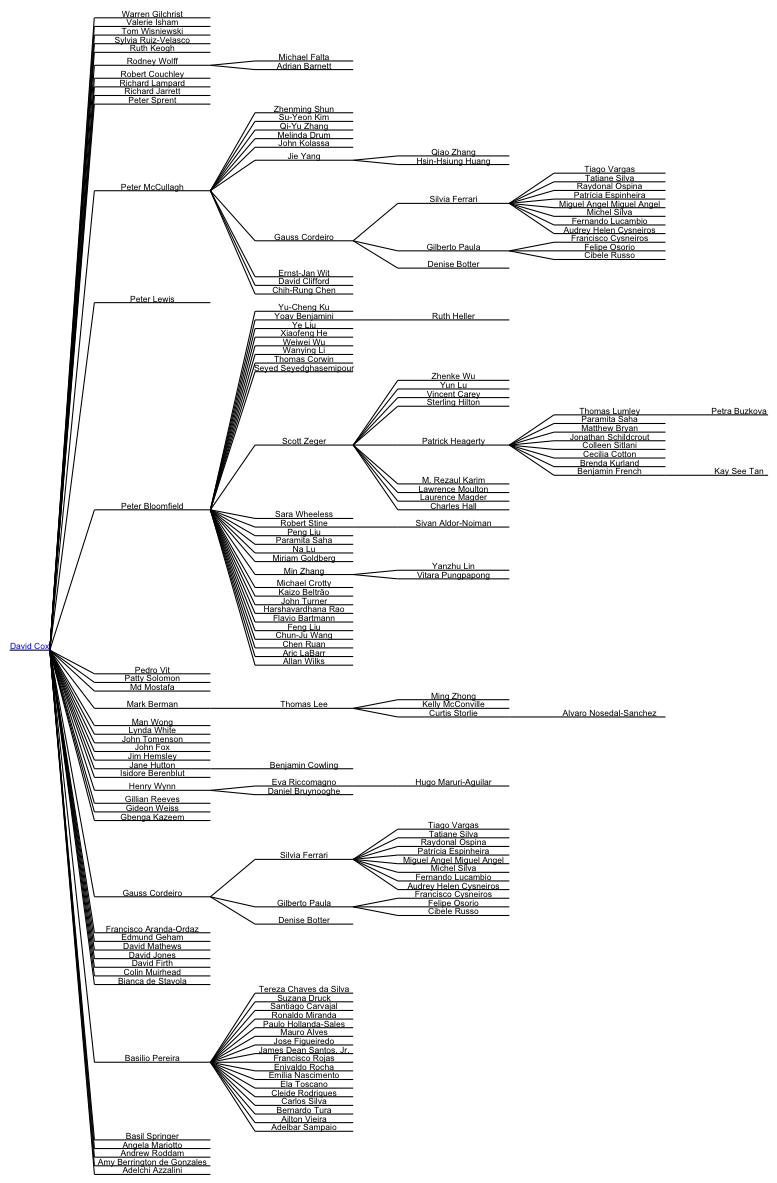
\includegraphics[width=\textwidth]{dCox.png}
    \caption{The 159 academic statistician ``descendants" of Sir David Cox.}
    \label{fig:dCox}
\end{figure}

We see from Figure \ref{fig:dCox} that Sir David Cox had 42 ``children", many of them becoming notable statisticians themselves, such as Basilio Pereira, Valerie Isham, Gauss Cordeiro, Peter McCullagh, and Henry Wynn. Of his ``children", the one who produced the most ``children" of their own was Peter Bloomfield, who has 26 ``children" and 49 ``descendants". In total, Sir David Cox had five generations of academic statistics mentees in this dataset.

\begin{CodeChunk}
\begin{CodeInput}
R> length(getChild("Peter Bloomfield", statGeneal))
\end{CodeInput}
\begin{CodeOutput}
[1] 26
\end{CodeOutput}
\begin{CodeInput}
R> nrow(getDescendants("Peter Bloomfield", statGeneal, gen = 100))
\end{CodeInput}
\begin{CodeOutput}
[1] 49
\end{CodeOutput}
\end{CodeChunk}

At this point, it would be insightful to examine a more detailed view of one of the longest strings of ``parent-child" relationships between Sir David Cox and one of the two individuals who are his fifth generation ``descendants". We do so with the code below, choosing his fifth generation ``descendant" to be Petra Buzkova. We set the \code{fontFace} variable of the \code{plotPath()} to a value of 4, indicating we wish to boldface and italicize the two varieties of interest.

\begin{CodeChunk}
\begin{CodeInput}
R> statIG <- dfToIG(statGeneal)
R> pathCB <- getPath("David Cox", "Petra Buzkova", statIG, statGeneal,
  isDirected = FALSE)
R> plotPath(pathCB, fontFace = 4) + ggplot2::theme(axis.text =
   ggplot2::element_text(size = 10), axis.title =
   ggplot2::element_text(size = 10))
\end{CodeInput}
\end{CodeChunk}

\begin{figure}[H]
    \centering
    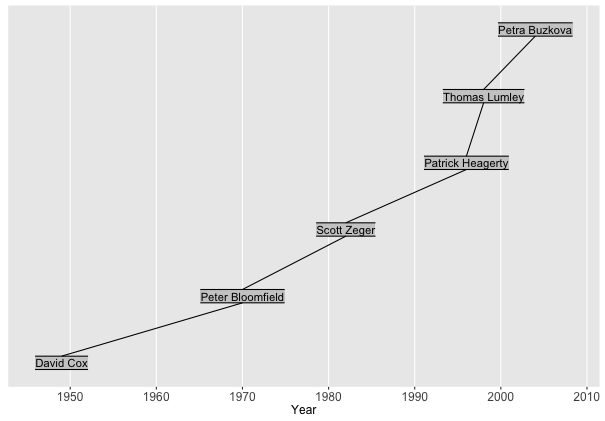
\includegraphics[width=0.7\textwidth]{pathCB}
    \caption{The shortest path between Sir David Cox and one of his fifth generation ``descendants", Petra Buzkova.}
    \label{fig:pathCB}
\end{figure}

This code results in Figure \ref{fig:pathCB}. We see that the shortest path between Sir David Cox and Petra Buzkova is strictly composed of five unidirectional ``parent-child" relationships that span about 55 years. We see that the time difference between when an advisor and student earned their degrees is not consistent across this path: The three statisticians who earned their degrees earliest in this path span more than 30 years in degree acquisition, whereas the three statisticians who earned their degrees later in this path only span less than ten years in degree acquisition.

We also notice in Figure \ref{fig:pathCB} that Sir David Cox received his statistics degree in about 1950, and Petra Buzkova received her statistics degree in about 2005. This genealogy only contains historical information about obtained degrees, and does not project into the future. Hence, we can be assured that Petra Buzkova is one of the younger individuals in the dataset, at least in the sense that the youngest individual could only have received his or her degree ten years after Petra Buzkova. However, we cannot be assured that Sir David Cox is one of the oldest individuals in the dataset. As such, it would be informative to superimpose this path of interest onto the entire dataset, using the \code{plotPathOnAll()} function of the \pkg{ggenealogy} package, as we did for the soybean genealogy in Figures \ref{fig:plotTNBin3} and \ref{fig:plotTNBin6}.

We can achieve this using the below code. After trial and error, we use a \code{binVector} of size 200, and append \pkg{ggplot2} syntax to define suitable x-axis limits. The output of this process is illustrated in Figure \ref{fig:plotCBText}.

\begin{CodeChunk}
\begin{CodeInput}
R> plotPathOnAll(pathCB, statGeneal, statIG, binVector = 1:200) +
   ggplot2::theme(axis.text = ggplot2::element_text(size = 8), axis.title =
   ggplot2::element_text(size = 8)) + ggplot2::scale_x_continuous
   (expand = c(.1, .2))
\end{CodeInput}
\end{CodeChunk}

\begin{figure}[H]
    \centering
    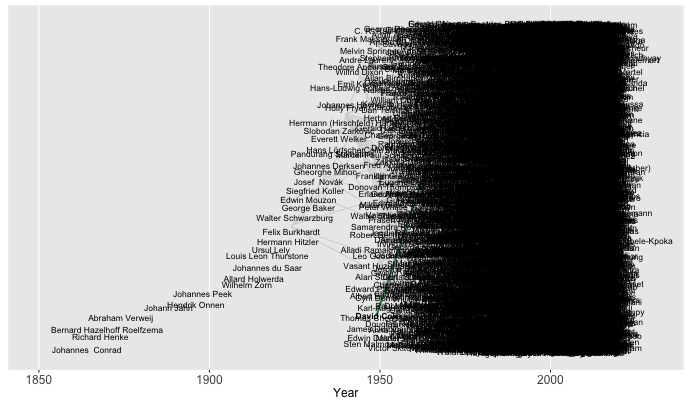
\includegraphics[width=\textwidth]{plotCBText}
    \caption{The shortest path between Sir David Cox and Petra Buzkova, superimposed over the data structure, using a bin size of 200.}
    \label{fig:plotCBText}
\end{figure}

We see from the resulting Figure \ref{fig:plotCBText} that almost all text labels for individuals who received their graduate-level statistics degrees between 1950 and 2015 are undecipherable. We also see that the year Sir David Cox acquired his statistics degree is somewhere in the later half of the variable year for this dataset, as the oldest dates for acquisition of statistics degrees in this dataset occur around 1860. However, the number of individuals who are documented as receiving their statistics degrees between 1860 and 1950 are few enough so that their text labels are somewhat readable.

The text labels are so numerous in Figure \ref{fig:plotCBText} that simply trying different values for the input parameter \code{binVector} will not solve the text overlapping problem. Instead, one approach we can try is to reconstruct the plot using the same \pkg{ggenealogy} function \code{plotPathOnAll()}, only now specifying variables to render the size (2.5) and color (default of black) of the text for nodes that are on the path of interest to be more noticeable than the size (0.5) and color (dark gray) of the text for nodes that are not on the path of interest. Moreover, we can make the edges that are not on the path of interest to be represented in a less noticeable color (light gray) than the edges that are on the path of interest (default of dark green). The variable names and options for these aesthetics is further detailed in the help manual of the function. We provide one example code that alters the defaults of the text color and sizes of nodes and edges below, which results in Figure \ref{fig:plotCBNoText}.

\begin{CodeChunk}
\begin{CodeInput}
R> plotPathOnAll(pathCB, statGeneal, statIG, binVector = 1:200, nodeSize = .5,
   pathNodeSize = 2.5, nodeCol = "darkgray", edgeCol = "lightgray") +
   ggplot2::theme(axis.text = ggplot2::element_text(size = 8), axis.title =
   ggplot2::element_text(size = 8)) + ggplot2::scale_x_continuous
   (expand = c(.1, .2))
\end{CodeInput}
\end{CodeChunk}

\begin{figure}[H]
    \centering
    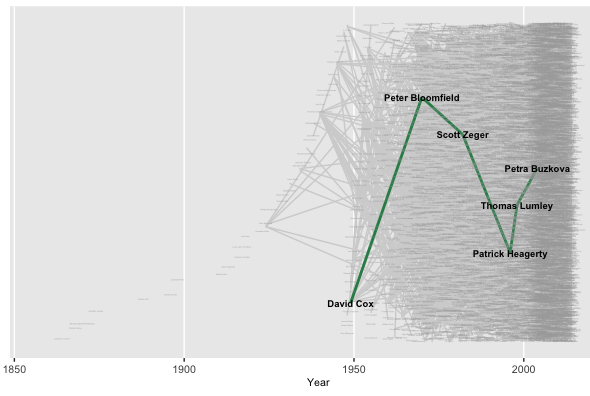
\includegraphics[width=\textwidth]{plotCBNoText}
    \caption{The shortest path between Sir David Cox and Petra Buzkova, superimposed over the data structure, using a bin size of 200. Individuals on the shortest path are labeled in large and black text and connected by dark green edges; all other individuals are labeled in small and gray text and connected by light gray edges.}
    \label{fig:plotCBNoText}
\end{figure}

In Figure \ref{fig:plotCBNoText}, we can now see each individual on the path of interest, and how their values for the variable year are overlaid on the entire genealogy structure. We can also more clearly see that, even though only ten years span between the youngest individual in the genealogy and Petra Buzkova, there are many individuals in that last decade. Indeed, the decade from 2005 to 2015 appears to be the densest in this dataset in terms of acquisition of statistics degrees.

We could still improve upon Figure \ref{fig:plotCBNoText}. Even though we may be primarily interested in understanding how the path of interest is overlaid across the entire genealogical structure, we could, upon viewing the entire structure, also develop an interest in nodes that are not on the path of interest but are revealed to stand out among the rest of the genealogical structure. For instance, in Figure \ref{fig:plotCBNoText}, it may be of interest for us to determine the names of the few individuals who obtained their statistics degrees before 1900. Fortunately, within the \code{plotPathOnAll()} function, there is a variable \code{animate} that we can set to a value of TRUE to create an interactive version of the figure that allows us to hover over individual illegible labels and immediately receive their labels in a readable format. A short video demonstration of these interactive features can be viewed upon clicking on Figure \ref{fig:plotAnimate}. 

\begin{CodeChunk}
\begin{CodeInput}
R> plotPathOnAll(pathCB, statGeneal, statIG, binVector = 1:200, nodeSize = .5,
   pathNodeSize = 2.5, nodeCol = "darkgray", edgeCol = "lightgray", animate =
   TRUE)
\end{CodeInput}
\end{CodeChunk}

\begin{figure}[H]
    \centering
    \includemedia[label = v1, playbutton=none, width=1.0\textwidth, addresource=animateGen.mov, activate=pageopen, flashvars={source=animateGen.mov}]{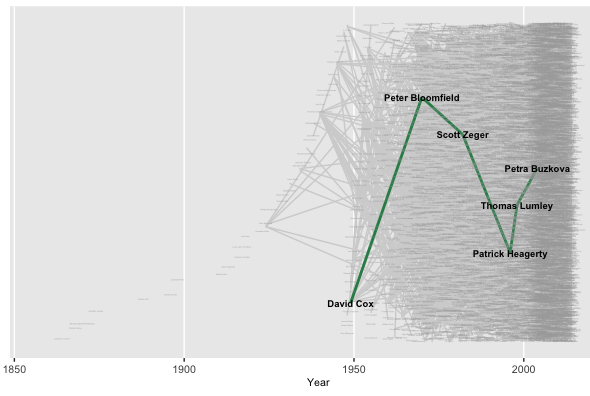
\includegraphics{./plotCBNoText.png}}{VPlayer.swf}
    \mediabutton[
mediacommand=v1:playPause,
]{\mybox{Play/Pause}}
    \caption{Upon clicking on this figure twice, a short video demonstrating the animation features for this function can be viewed. Please note that to properly view this video, the PDF version of this paper must be opened in Adobe Acrobat Reader DC, which can be downloaded free of charge.}
    \label{fig:plotAnimate}
\end{figure}

\section{Future Avenues}

Incorporation of the Shiny application allows users to examine \pkg{ggenealogy} tools in a more interactive way (\citealt{shiny}). The reactive programming saves them the time of using command-line for each change of input as well as the inefficiency of rerunning code. A Shiny application that uses certain \pkg{ggenealogy} functionality is available for users who wish to explore the soybean genealogy; the data can be viewed at \url{http://shiny.soybase.org/CNV/}.

We also aim to incorporate plotting tools that can examine not only quantitative variables (such as our example variable of ``year"), but also categorical variables associated with individuals in datasets. Moreover, we look forward to testing the \pkg{ggenealogy} package on additional genealogical data sets. Exploring several datasets with the software will allow us to fix remaining bugs, and provide us further insight into how to make our tools available for a wide range of data input formats. 

The \pkg{ggenealogy} visualization tool \code{plotPathOnAll()} is suitable as a data exploration tool, but not always as a publication tool. This is because we still see textual overlap in small-enough datasets (see Figure \ref{fig:plotTNBin6}). As such, we plan to add a feature to the package that allows users to manually fine-tune automated plots. For example, after comparing several bin sizes on the soybean genealogy, we determined that the bin size of 6 produced the minimal textual overlap, as is seen in Figure \ref{fig:plotTNBin6}. If we could subsequently fine-tune the vertical positions of the small fraction of text labels that remained overlapped after the automated \pkg{ggenealogy} function, then we could potentially remove all overlaps, and the plot could be used in presentations and publications. Of course, it is impossible to eliminate textual overlap in larger datasets (see Figure \ref{fig:plotCBText}). In such cases, we can remedy this problem by representing individuals who are not on the path of interest with dots instead of text (see Figure \ref{fig:plotCBNoText}).

\section{Conclusions}

The \pkg{ggenealogy} package offers various plotting tools that can assist those studying genealogical lineages in the data exploration phases, as well as in preparing publication-suitable images. As each plot comes with its pros and cons, we recommended for users to explore several visualization tools. If users are simultaneously using similar packages, we in particular recommend using the \code{plotAncDes()} function. This plot allows users to view generation counts of a variety of interest in a manner that is not as readily available in similar software packages.

\section*{Acknowledgments}

The authors thank Drs. James E. Specht and Randy C. Shoemaker for helpful discussions of soybean genealogy. In addition, the authors are grateful for the financial support from the United Soybean Board (Project 1204), The North Central Soybean Research Program, the NSF Plant Genome Research Program (award number 0820642), and the USDA-ARS CRIS Project 3625-21220-005-00D. The USDA is an equal opportunity provider and employer. Mention of trade names or commercial products in this article is solely for the purpose of providing specific information and does not imply recommendation or endorsement by the U.S. Department of Agriculture. Author Cook was a faculty member at Iowa State University at the time that most of this work was conducted.

\bibliography{article}

\end{document}
